\begin{abstract}
Glaucoma is a leading cause of irreversible blindness, and automated screening from fundus photographs is attractive, but results are hard to interpret when images from several sources are pooled. We study normal versus glaucoma classification on 2,468 images from three public datasets (ORIGA, G1020, and REFUGE), using 2,099 development images, with a held-out test set that is not used for any comparison. A development phase (grouped five-fold cross-validation, three seeds) compares ResNet50, DenseNet121, and EfficientNet-B0, with and without pretraining on a second public fundus dataset (ODIR). A final protocol (grouped ten-fold cross-validation, five seeds per fold) then compares a configuration fixed in advance, an equal-weight ensemble of 20 EfficientNet-B0 models (ODIR-pretrained at 224 pixels and ImageNet-initialized at 384 pixels), with a ResNet50 baseline. The ensemble reaches a pooled out-of-fold ROC-AUC of 0.774 (95\% bootstrap interval 0.752 to 0.796) against 0.742 for ResNet50, a paired difference of $+0.032$ (0.015 to 0.049) with a higher fold score in 7 of 10 folds. Part of this gain comes from ensemble size, the gain from ODIR pretraining depends on the pretraining run, and the configuration was fixed after the development scores were known, so the selection is not blind. A per-source analysis shows that the pooled score hides a large difference: ROC-AUC is 0.82 on ORIGA and 0.94 on REFUGE, but at chance level (0.50) on G1020. We report all negative and inconclusive results and recommend that per-source scores accompany pooled scores for multi-source fundus data.
\end{abstract}

\begin{IEEEkeywords}
Cross-validation, deep learning, ensemble learning, fundus images, glaucoma, transfer learning.
\end{IEEEkeywords}

\section{Introduction}
\label{sec:intro}
\IEEEPARstart{G}{laucoma} is a progressive optic neuropathy and a leading cause of irreversible blindness. An estimated 64.3 million people aged 40 to 80 years were affected in 2013, and the number is projected to exceed 110 million by 2040 \cite{tham2014}. Because early disease is usually without symptoms, screening with color fundus photography is attractive, and many deep learning systems have been proposed to classify fundus images as normal or glaucomatous.

Reported accuracies in this literature are often high, but they are rarely comparable. Studies differ in the task (binary screening, stage grading, or optic disc and cup segmentation), in the data (a single private hospital collection, or a single public dataset), and in the protocol (random image-level splits, balancing by augmentation, or the choice of model settings on the same folds that are reported). Several public datasets contain more than one photograph of the same eye, so a random split can place near-identical images in both the training and the test part. Pooling datasets from different cameras and labeling conventions makes the task harder, and a single pooled score then hides how the model behaves on each source.

This paper takes the opposite approach: a deliberately strict evaluation of a standard transfer learning pipeline on three public datasets pooled together. Our contributions are as follows.
\begin{enumerate}
\item We build a leakage-controlled benchmark of 2,468 fundus images from ORIGA, G1020, and REFUGE, in which near-duplicate images of the same eye are grouped and never separated across splits, and one pair of images with conflicting labels is removed.
\item We evaluate ResNet50, DenseNet121, and EfficientNet-B0 with grouped cross-validation, several training seeds per fold, and group bootstrap confidence intervals, in a development phase (five folds, three seeds) and in a final protocol (ten folds, five seeds), and we keep a held-out test set out of every comparison.
\item We test whether pretraining on a second public fundus dataset (ODIR) improves transfer, using three independent pretraining runs, and we report that the gain is modest and depends on the pretraining run.
\item We fix a final configuration by a written rule before the final run and compare it with a ResNet50 baseline in the same protocol: a pooled ROC-AUC of 0.774 against 0.742, a paired difference of $+0.032$ with a 95\% interval of 0.015 to 0.049. We state which part of this gain may come from ensemble size, and that the selection was not blind.
\item We report performance per source and show that a pooled score combines good results on ORIGA (0.82) and REFUGE (0.94) with chance-level results on G1020 (0.50), and we examine one candidate explanation.
\end{enumerate}
We do not claim to outperform published systems, whose tasks and protocols differ from ours (Section~\ref{sec:related}). Our aim is an honest estimate of what a standard pipeline achieves under strict, multi-source evaluation.


\section{Related Work}
\label{sec:related}
\subsection{Handcrafted Features}
Early automated systems extracted handcrafted features and used classical classifiers. Maheshwari \emph{et al.}\ \cite{maheshwari2017} decomposed fundus images with the empirical wavelet transform, extracted correntropy features, and classified them with a least-squares support vector machine. They report accuracies of 98.33\% (3-fold) and 96.67\% (10-fold) on a private set of 60 images, but about 81\% on a public set of 505 images, and the kernel settings were chosen to give the highest accuracy. Parashar and Agrawal \cite{parashar2021a,parashar2021b,parashar2020} used variational mode decomposition, the tensor empirical wavelet transform, and the flexible analytic wavelet transform, followed by entropy or texture features and support vector machine classifiers, to grade glaucoma stages. With 10-fold cross-validation on datasets of a few hundred to about 900 images, they report accuracies from 93\% to 98\%.

\subsection{Deep Learning and Attention}
Convolutional networks learn features directly from images. Das \emph{et al.}\ \cite{das2023} proposed CA-Net, a cascaded attention module on a DenseNet121 backbone for three-stage classification (normal, early, and advanced glaucoma), evaluated with a single 70:30 split on two datasets of about 1,500 images each and reporting accuracies of 85.34\% and 83.85\%. Yi \emph{et al.}\ \cite{yi2023} proposed MTRA-CNN, which pretrains ResNet50 first on ImageNet and then on the ODIR dataset before fine-tuning on a private four-class grading set, with 10-fold cross-validation and 86.8\% accuracy. This idea of same-domain fundus pretraining is the one we test in the binary setting, with a pre-registered success rule.

Das \emph{et al.}\ \cite{das2026} proposed MixWT-Net, which combines a DenseNet121 backbone, a module that mixes feature statistics (MixStyle), and a wavelet-based efficient self-attention module. It reaches 98.46\% accuracy on a random 70:30 split of the LAG dataset and is then tested without retraining on ORIGA, REFUGE, and Drishti-GS, where accuracy falls to 78.61\%, 86.75\%, and 82.17\% (area under the curve 0.771, 0.886, and 0.876). This is the closest published comparison to our data, because it uses two of our three datasets, but its protocol (training on a different dataset and testing on each of ours) differs from ours. Abay \emph{et al.}\ \cite{abay2026} screened for glaucoma with a lightweight network on frames from low-cost smartphone fundus videos, locating the optic disc first. With subject-level cross-validation on 227 frames they report an accuracy of 97.86\%, and on a held-out set of 57 frames (14 glaucoma) an accuracy of 89.5\% and an area under the curve of 0.906. Preity \emph{et al.}\ \cite{preity2026} segment the optic disc and cup and derive clinical rules, so their reported pixel accuracies of up to 99.4\% measure segmentation rather than image-level diagnosis.

\subsection{Summary}
Table~\ref{tab:related} summarizes these studies. The reported numbers fall from above 97\% to about 78 to 90\% when testing moves from a random split of one dataset, or a small private set, to an external or held-out set. We therefore evaluate with grouped cross-validation on pooled data and report performance for each source.

\begin{table*}[!t]
\caption{Summary of Related Studies (Numbers as Reported by the Authors)}
\label{tab:related}
\centering
\footnotesize
\begin{tabular}{p{2.3cm}p{2.6cm}p{4.6cm}p{3.0cm}p{3.7cm}}
\toprule
Study & Task & Data & Protocol & Reported result \\
\midrule
Maheshwari \cite{maheshwari2017} & Normal vs.\ glaucoma & Private 60 images; public 505 images & 3-fold and 10-fold CV & Private 98.33\%/96.67\%; public 81.32\%/80.66\% accuracy \\
Yi \cite{yi2023} & Four-class grading & Private hospital set (492, 297, 173, 306 images), balanced by augmentation & 10-fold CV & Accuracy 86.8\%, AUC 0.91 \\
Das \cite{das2023} & Three-stage grading & Harvard Dataverse V1 (1,542) and LMG (1,582) images & Single 70:30 split & Accuracy 85.34\% and 83.85\% \\
Das \cite{das2026} & Normal vs.\ glaucoma, cross-dataset & Train: LAG (4,854); test: ORIGA (650), REFUGE (400), Drishti-GS (101) & LAG random 70:30; others zero-shot & LAG 98.46\%; ORIGA 78.61\%, REFUGE 86.75\%, Drishti 82.17\% accuracy \\
Abay \cite{abay2026} & Normal vs.\ glaucoma, smartphone video & Own clinical data, 227 frames; held-out 57 frames & Subject-level 5-fold CV; held-out set & CV 97.86\%; held-out 89.5\% accuracy, AUC 0.906 \\
Parashar \cite{parashar2021a,parashar2021b,parashar2020} & Three-stage grading & Small public and private sets (about 270 to 900 images) & 10-fold CV & Accuracy 93\% to 98\% \\
Preity \cite{preity2026} & Disc and cup segmentation & DRISHTI, RIM-ONE, ORIGA, REFUGE & Per dataset and cross-dataset & Pixel accuracy up to 99.4\% \\
This work & Normal vs.\ glaucoma, pooled & ORIGA, G1020, REFUGE (2,099 development images) & Grouped 10-fold CV, 5 seeds, bootstrap CIs & AUC 0.774 (ResNet50 0.742); per source 0.82 / 0.94 / 0.50 \\
\bottomrule
\end{tabular}
\end{table*}

\section{Datasets and Preprocessing}
\label{sec:data}
\subsection{Datasets}
We classify fundus images as normal or glaucoma using three public datasets: ORIGA \cite{zhang2010}, G1020 \cite{bajwa2020}, and REFUGE \cite{orlando2020}. The raw collection holds 2,470 images (1,926 normal, 544 glaucoma). After curation, 2,468 remain (1,925 normal, 543 glaucoma), a 78\% to 22\% class split. Table~\ref{tab:data} gives the composition of the 2,099 images used for model development.

\begin{table}[!t]
\caption{Composition of the Development Set (Train and Validation, 2,099 Images)}
\label{tab:data}
\centering
\footnotesize
\begin{tabular}{lrrr}
\toprule
Source & Images & Glaucoma & Glaucoma share \\
\midrule
ORIGA & 553 & 143 & 25.9\% \\
REFUGE (train and validation) & 680 & 68 & 10.0\% \\
G1020 & 866 & 251 & 29.0\% \\
Total & 2,099 & 462 & 22.0\% \\
\bottomrule
\end{tabular}
\end{table}

\subsection{Duplicates and Splits}
An exact (MD5) check found no identical files. A perceptual-hash check (nearest neighbor, confirmed by a pixel mean absolute error below 5.0) found eight pairs that appear to show the same eye photographed on different occasions. One pair, both from G1020, carried conflicting labels (one image normal, one glaucoma). We could not tell which label was correct, so we excluded both images rather than guess. The other seven pairs were treated as groups that are never separated across splits.

The data were split 70/15/15 into training, validation, and test sets (1,729, 370, and 369 images), stratified by source and class, with no group crossing a split. The test set (369 images, 81 with glaucoma) was not used for any comparison reported here; it was opened twice earlier, each time for a single ResNet50 model, as stated in the limitations. All comparisons use only the 2,099 training and validation images, in grouped cross-validation (Section~\ref{sec:protocol}).

\subsection{Preprocessing}
Each image is converted to the YUV color space, contrast-limited adaptive histogram equalization (clip limit 2.0, 8 by 8 tiles) is applied to the luminance channel only \cite{zuiderveld1994}, and the image is converted back to RGB. This is done at full resolution, after which the shorter side is resized to 256 pixels for 224-pixel models, or to 440 pixels for 384-pixel models. Training uses a random crop, horizontal flip (no vertical flip), rotation of up to 15 degrees, and color jitter. Evaluation uses a center crop. Inputs are normalized with ImageNet statistics, and class weights come from the training class counts.

\section{Methods}
\label{sec:methods}
We use transfer learning from ImageNet \cite{deng2009} with one fixed training recipe, applied to three backbones in the development phase: ResNet50 \cite{he2016}, DenseNet121 \cite{huang2017}, and EfficientNet-B0 \cite{tan2019}. The final protocol uses ResNet50 and EfficientNet-B0. The recipe was designed on ResNet50 and was not re-tuned for the other backbones or for other image sizes.

\subsection{Two-Phase Training}
Phase A trains only the new two-class head (Adam \cite{kingma2015}, learning rate $10^{-3}$, up to 15 epochs). Phase B unfreezes the later backbone stages and continues (backbone learning rate $10^{-4}$, head learning rate $10^{-3}$, up to 20 epochs). Both phases use a class-weighted cross-entropy loss, batch size 32, mixed precision, a plateau-based learning-rate schedule (patience 3), and early stopping (patience 6). The phase with the lower validation loss is kept. Validation here is an inner split of about 14\% of each fold's training part, so the held-out fold is never used for any choice. Models are trained at 224 pixels, and EfficientNet-B0 is also trained at 384 pixels.

\subsection{Pretraining on a Second Fundus Dataset}
For the ODIR arms we first pretrain EfficientNet-B0 (224 pixels) on the public ODIR dataset \cite{odir2019}, using per-eye labels: eyes whose only diagnostic keyword is glaucoma (196 eyes) are positive, eyes whose only keyword is normal fundus (2,735 eyes) are negative, and all other eyes are dropped. The 2,931 eyes are split by patient into training and validation parts (2,512 and 419 eyes for seeds 42 and 7, 2,514 and 417 for seed 123), and early stopping uses only the validation part. ODIR images are compared with every project image, including the test images, by perceptual hash. Candidates that matched test images (141) were dropped as a precaution, although a pixel comparison showed that none was a true duplicate. Only the backbone weights are saved, and the classifier head is re-initialized for the glaucoma task. We ran three independent pretraining runs (seeds 42, 7, and 123) and report all three. The runs differ in the ODIR split as well as in the seed.

\subsection{Ensembling and the Final Configuration}
A seed ensemble averages the predicted probabilities of the models trained with different seeds on the same fold: three seeds (101, 202, and 303) in the development phase and five seeds (101, 202, 303, 404, and 505) in the final protocol. Cross-model ensembles average the probabilities of all models in the mix with equal weight per model. In the development phase the mixes were chosen after seeing the results, so they are exploratory.

Before running the final protocol we wrote down a rule for choosing the final configuration, using only the development results. The candidate with the highest mean ensemble ROC-AUC (a mix of 15 models, 0.7776) sets the benchmark. Every candidate within 0.005 of it counts as tied, and among the tied candidates the one with the lowest training cost is chosen. The rule also requires that any choice involving ODIR pretraining be based on at least three independent pretraining runs, all reported, and that whatever the final run shows is reported without changing the choice. Applied to the development table, the rule selects ODIR-pretrained EfficientNet-B0 at 224 pixels (three pretraining runs, seeds 42, 7, and 123) together with ImageNet-initialized EfficientNet-B0 at 384 pixels. We call this the \emph{final configuration}: four arms of five seeds each, 20 models per fold, averaged with equal weight. The ResNet50 recipe at 224 pixels, run in the same protocol, is the baseline. Because the development scores of all candidates were already known when the rule was written, the selection is not blind. The rule fixes the decision logic before the final run, so that the choice cannot change after the final numbers are seen, but it does not remove the possibility that the final configuration benefits from having been picked among well-performing options.

\section{Evaluation Protocol}
\label{sec:protocol}
Both phases use grouped cross-validation on the 2,099 development images (2,093 groups, none split across folds, fold seed 42). Every model sees exactly the same held-out images in every fold, and the code asserts this. The development phase uses five folds and three training seeds per fold. The final protocol uses ten folds (209 to 211 images each, with 33 to 55 glaucoma images per fold) and five training seeds per fold, and all five arms (the three ODIR arms, the 384-pixel arm, and the ResNet50 baseline) share the same folds. In the final protocol every model is trained on about nine tenths of the development images, of which about 14\% form an inner validation split used for early stopping, for choosing between the two training phases, and for choosing thresholds, so the held-out fold is never used for any choice.

\textit{Metrics.} The primary metric is the area under the receiver operating characteristic curve (ROC-AUC), computed on the pooled out-of-fold predictions and, as a check, per fold (mean and standard deviation across folds, with $n-1$ in the denominator). The area under the precision-recall curve (PR-AUC) is a second metric because glaucoma is the minority class. For the operating points, each fold's threshold is set on that fold's inner validation split, either by the Youden index or as the quantile of inner-validation normal images that gives a target specificity, and is then applied to the held-out fold. Counts are pooled over the ten folds.

\textit{Uncertainty.} Confidence intervals come from a bootstrap that resamples groups (1,000 resamples). The same resamples are used for every model, so differences between models are paired. The trained models are held fixed, so these intervals reflect sampling of the evaluation images only and not training randomness. For that reason we also report in how many folds a method wins, which is closer to a test of consistency.

\textit{Pre-registered rule for ODIR (development phase).} Before running any ODIR experiment we fixed the criteria for calling the ODIR gain real: a mean ensemble ROC-AUC gain of at least 0.010 over ImageNet-only EfficientNet-B0 at 224 pixels, a better score in at least four of five folds, and a paired bootstrap interval that excludes zero. We applied the same criteria to the first two pretraining runs.

\section{Results}
\label{sec:results}
\subsection{Development Phase (Five Folds, Three Seeds)}
Every single configuration scores about 0.75 to 0.77 cross-validated ROC-AUC. Seed ensembling, higher resolution, and ODIR pretraining each add a small amount, and the gains are smaller than the fold-to-fold spread unless stated. Table~\ref{tab:single} gives the single-configuration results.

\begin{table*}[!t]
\caption{Development Phase: Single Configurations (Ensemble = Mean of Three Training Seeds; Mean $\pm$ Standard Deviation Over Five Folds)}
\label{tab:single}
\centering
\footnotesize
\begin{tabular}{lcccc}
\toprule
Configuration & Single ROC-AUC & Ensemble ROC-AUC & Ensemble PR-AUC & Pooled ensemble ROC-AUC [95\% CI] \\
\midrule
ResNet50, 224 px & 0.7353 & 0.7500 $\pm$ 0.0202 & 0.4345 & 0.7472 [0.7240, 0.7690] \\
DenseNet121, 224 px & 0.7328 & 0.7468 $\pm$ 0.0142 & 0.4364 & 0.7463 [0.7246, 0.7675] \\
EfficientNet-B0, 224 px, ImageNet & 0.7448 & 0.7561 $\pm$ 0.0104 & 0.4469 & 0.7552 [0.7321, 0.7772] \\
EfficientNet-B0, 384 px, ImageNet & 0.7577 & 0.7635 $\pm$ 0.0184 & 0.4808 & 0.7641 [0.7411, 0.7864] \\
EfficientNet-B0, 224 px, ODIR pretraining, seed 42 & 0.7655 & 0.7736 $\pm$ 0.0250 & 0.4852 & 0.7749 [0.7521, 0.7957] \\
EfficientNet-B0, 224 px, ODIR pretraining, seed 7 & 0.7518 & 0.7618 $\pm$ 0.0098 & 0.4719 & 0.7599 [0.7371, 0.7805] \\
\bottomrule
\end{tabular}
\end{table*}

\textit{Backbones.} The three backbones cannot be told apart. EfficientNet-B0 minus ResNet50 is $+0.0078$ pooled ROC-AUC (95\% CI $-0.0104$ to $+0.0265$), so a 4M-parameter model matches the 23.5M-parameter ResNet50. Seed ensembling added about $+0.011$ to $+0.015$ ROC-AUC over a single model on every backbone at 224 pixels.

\textit{Resolution.} At 384 pixels, EfficientNet-B0 gains $+0.0074$ ensemble ROC-AUC over 224 pixels on the fold mean, with a better score in three of five folds (pooled $+0.0090$, CI $-0.0069$ to $+0.0248$). That is not a clear win, although PR-AUC rises by 0.034, and training costs about 2.5 times more.

\textit{ODIR pretraining.} Under the pre-registered rule, pretraining run 42 passed ($+0.0175$ over ImageNet-only at 224 pixels, better in four of five folds, pooled $+0.0195$, CI $+0.0064$ to $+0.0326$). Pretraining run 7 did not ($+0.0057$, better in three of five folds, pooled $+0.0044$, CI $-0.0062$ to $+0.0160$). The two runs differ from each other by $-0.0151$ pooled (run 7 minus run 42, CI $-0.0271$ to $-0.0025$), which is why the final protocol uses three runs.

\textit{Exploratory ensembles.} Mixing models of different architectures, resolutions, or initializations helps more than any single change (Table~\ref{tab:mix}). These mixes were assembled after seeing the results, and the intervals treat the trained models as fixed, so Table~\ref{tab:mix} is exploratory. The mixes level off near 0.777 to 0.778, and they are the evidence on which the final configuration was chosen (Section~\ref{sec:methods}).

\begin{table*}[!t]
\caption{Development Phase: Mixed Ensembles (Exploratory)}
\label{tab:mix}
\centering
\footnotesize
\begin{tabular}{lccc}
\toprule
Ensemble & Models & Ensemble ROC-AUC & Pooled ROC-AUC [95\% CI] \\
\midrule
EfficientNet-B0 224 + 384 & 6 & 0.7692 $\pm$ 0.0085 & 0.7698 [0.7469, 0.7915] \\
ResNet50 + DenseNet121 + EfficientNet-B0 (224 px) & 9 & 0.7693 $\pm$ 0.0051 & 0.7676 [0.7461, 0.7889] \\
Those three + EfficientNet-B0 384 & 12 & 0.7726 $\pm$ 0.0074 & 0.7728 [0.7508, 0.7943] \\
ODIR seed 42 + EfficientNet-B0 384 & 6 & 0.7771 $\pm$ 0.0193 & 0.7791 [0.7574, 0.8006] \\
ODIR seeds 42 and 7 + EfficientNet-B0 384 & 9 & 0.7769 $\pm$ 0.0158 & 0.7782 [0.7564, 0.7988] \\
ResNet50, DenseNet121, EfficientNet-B0 224 and 384, ODIR seed 42 & 15 & 0.7776 $\pm$ 0.0110 & 0.7780 [0.7561, 0.7985] \\
Same five plus ODIR seed 7 & 18 & 0.7776 $\pm$ 0.0103 & 0.7776 [0.7558, 0.7984] \\
\bottomrule
\end{tabular}
\end{table*}

\subsection{Final Protocol (Ten Folds, Five Seeds)}
Table~\ref{tab:final} gives the results of the final protocol, and Fig.~\ref{fig:roc} shows the pooled ROC curves. The final configuration (20 models) reaches a pooled out-of-fold ROC-AUC of 0.7743 (95\% CI 0.7525 to 0.7959) and a fold mean of $0.7763 \pm 0.0234$, against 0.7420 (0.7173 to 0.7650) and $0.7473 \pm 0.0420$ for the ResNet50 baseline. PR-AUC is 0.471 against 0.411. Every arm scores between 0.755 and 0.773, and the ResNet50 baseline has the lowest score of the five.

\begin{table*}[!t]
\caption{Final Protocol: Out-of-Fold Results (Ten Folds, Five Seeds per Arm; Arm Ensemble = Mean of Five Seeds)}
\label{tab:final}
\centering
\footnotesize
\begin{tabular}{lccccc}
\toprule
Arm & Models & Single-seed ROC-AUC & Fold mean $\pm$ SD & Pooled ROC-AUC [95\% CI] & Pooled PR-AUC [95\% CI] \\
\midrule
ResNet50, 224 px, ImageNet (baseline) & 5 & 0.7234 & 0.7473 $\pm$ 0.0420 & 0.7420 [0.7173, 0.7650] & 0.411 [0.370, 0.458] \\
EfficientNet-B0, 384 px, ImageNet & 5 & 0.7511 & 0.7640 $\pm$ 0.0313 & 0.7620 [0.7398, 0.7832] & 0.456 [0.412, 0.502] \\
EfficientNet-B0, 224 px, ODIR run 42 & 5 & 0.7645 & 0.7727 $\pm$ 0.0296 & 0.7727 [0.7507, 0.7939] & 0.477 [0.431, 0.525] \\
EfficientNet-B0, 224 px, ODIR run 7 & 5 & 0.7444 & 0.7552 $\pm$ 0.0368 & 0.7550 [0.7344, 0.7787] & 0.432 [0.388, 0.484] \\
EfficientNet-B0, 224 px, ODIR run 123 & 5 & 0.7518 & 0.7635 $\pm$ 0.0187 & 0.7602 [0.7374, 0.7833] & 0.458 [0.414, 0.511] \\
ODIR average (three runs) & 15 & --- & 0.7703 $\pm$ 0.0275 & 0.7696 [0.7473, 0.7915] & 0.465 [0.421, 0.516] \\
\textbf{Final configuration} & 20 & --- & 0.7763 $\pm$ 0.0234 & 0.7743 [0.7525, 0.7959] & 0.471 [0.426, 0.521] \\
\bottomrule
\end{tabular}
\end{table*}

\begin{figure}[!t]
\centering
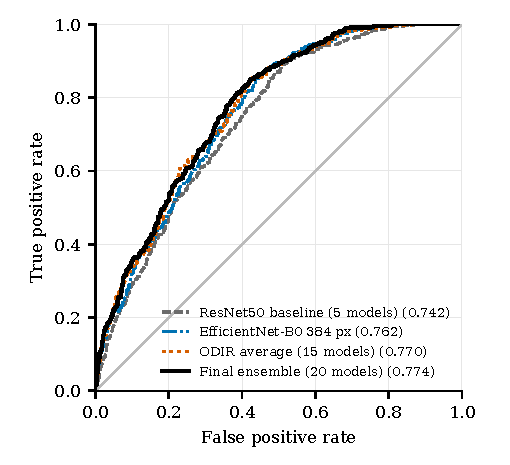
\includegraphics[width=\columnwidth]{figs/fig_roc.pdf}
\caption{Pooled out-of-fold ROC curves on the 2,099 development images (final protocol). The pooled ROC-AUC of each is given in parentheses. The curves overlap over much of their length.}
\label{fig:roc}
\end{figure}

\textit{Paired comparison with the baseline.} Because all arms share folds and bootstrap resamples, differences can be paired (Table~\ref{tab:paired}). The final configuration is $+0.0323$ above ResNet50 in pooled ROC-AUC (95\% CI $+0.0154$ to $+0.0490$), with a mean fold difference of $+0.0291 \pm 0.0370$ and a higher score in 7 of 10 folds. The ODIR average and the 384-pixel arm have intervals above zero as well. The arm with ODIR run 7 is the exception: its interval includes zero ($+0.0130$, $-0.0057$ to $+0.0320$).

\begin{table*}[!t]
\caption{Final Protocol: Difference From the ResNet50 Baseline (Paired)}
\label{tab:paired}
\centering
\footnotesize
\setlength{\tabcolsep}{3pt}
\begin{tabular}{lccc}
\toprule
Arm & Pooled difference [95\% CI] & Fold mean $\pm$ SD & Folds won \\
\midrule
ODIR run 42 & $+0.0307$ [$+0.0127$, $+0.0474$] & $+0.0255 \pm 0.0423$ & 7 \\
ODIR run 7 & $+0.0130$ [$-0.0057$, $+0.0320$] & $+0.0079 \pm 0.0491$ & 6 \\
ODIR run 123 & $+0.0182$ [$+0.0008$, $+0.0364$] & $+0.0162 \pm 0.0377$ & 6 \\
EfficientNet-B0, 384 px & $+0.0200$ [$+0.0005$, $+0.0386$] & $+0.0168 \pm 0.0384$ & 8 \\
ODIR average (15 models) & $+0.0276$ [$+0.0105$, $+0.0445$] & $+0.0230 \pm 0.0422$ & 7 \\
Final configuration (20) & $+0.0323$ [$+0.0154$, $+0.0490$] & $+0.0291 \pm 0.0370$ & 7 \\
\bottomrule
\end{tabular}
\end{table*}

\textit{ODIR pretraining depends on the run.} The three pretraining runs give pooled scores of 0.7727, 0.7550, and 0.7602. Run 7 minus run 42 is $-0.0176$ (95\% CI $-0.0299$ to $-0.0041$) and run 123 minus run 42 is $-0.0125$ ($-0.0239$ to $-0.0009$), so run 42 is better than the other two even though all three use the same recipe and the same images. The ODIR average of 0.7696 is therefore the more honest estimate of what ODIR pretraining gives. Run 42 is also the run that passed the pre-registered rule in the development phase, and its fold-mean ensemble score in the final protocol (0.7727) is close to its development score (0.7736). We cannot say why one pretraining run is better than another.

\textit{Combining arms.} The final configuration is $+0.0047$ above the ODIR average (CI $+0.0010$ to $+0.0081$) and $+0.0123$ above the 384-pixel arm alone ($+0.0017$ to $+0.0234$). The 384-pixel arm is $-0.0076$ below the ODIR average, with an interval that includes zero ($-0.0222$ to $+0.0061$). The predicted probabilities of the three ODIR arms correlate at 0.92 with each other and at 0.86 with the 384-pixel arm, so combining the two kinds of models gives a small additional gain.

\subsection{Per-Source Performance}
Pooling hides how the models behave on each source. We computed the ROC-AUC separately for the out-of-fold predictions of each source, with group-level bootstrap intervals (Table~\ref{tab:source} and Fig.~\ref{fig:source}). Both the final configuration and the baseline show the same pattern: performance is good on REFUGE, moderate on ORIGA, and at chance level on G1020 (0.501 and 0.494, with both intervals containing 0.5). The final configuration is higher than the baseline on ORIGA (0.819 against 0.774) and on REFUGE (0.941 against 0.911), but the intervals overlap, so the per-source gains are suggestive rather than separate findings. The ordering of ORIGA and REFUGE agrees with the zero-shot results of Das \emph{et al.}\ \cite{das2026}, who also find ORIGA harder than REFUGE (area under the curve 0.771 versus 0.886).

\begin{table*}[!t]
\caption{Per-Source ROC-AUC of the Out-of-Fold Predictions [95\% Bootstrap CI]}
\label{tab:source}
\centering
\footnotesize
\setlength{\tabcolsep}{2.5pt}
\begin{tabular}{lcc}
\toprule
Source (images; glaucoma) & Final configuration & ResNet50 baseline \\
\midrule
ORIGA (553; 143) & 0.819 [0.779, 0.858] & 0.774 [0.729, 0.818] \\
REFUGE, all (680; 68) & 0.941 [0.911, 0.966] & 0.911 [0.873, 0.947] \\
\quad REFUGE train part (340; 34) & 0.900 [0.837, 0.956] & 0.864 [0.782, 0.938] \\
\quad REFUGE validation part (340; 34) & 0.971 [0.951, 0.988] & 0.944 [0.901, 0.978] \\
G1020 (866; 251) & 0.501 [0.462, 0.542] & 0.494 [0.450, 0.536] \\
\bottomrule
\end{tabular}
\end{table*}

\begin{figure}[!t]
\centering
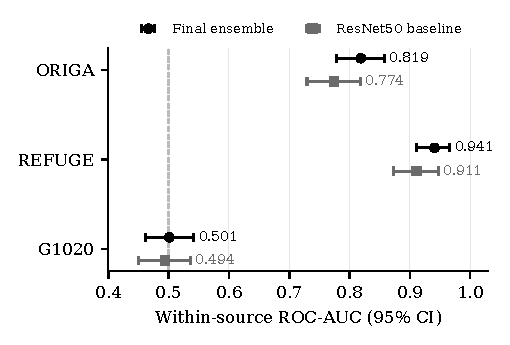
\includegraphics[width=\columnwidth]{figs/fig_source.pdf}
\caption{ROC-AUC within each source with 95\% bootstrap intervals (final protocol). The dashed line marks chance level. Both models are at chance level on G1020.}
\label{fig:source}
\end{figure}

\subsection{Operating Points}
A threshold turns the model's probability into a decision, and moving it trades sensitivity against specificity. Table~\ref{tab:op} shows the final configuration and the baseline at the balanced (Youden) threshold and at thresholds chosen on the inner validation split to reach a target specificity, with all metrics measured on the held-out folds and pooled over the ten folds. Accuracy rises as specificity is pushed up, but only because about 78\% of the images are normal: a classifier that called every image normal would score about 78\% accuracy and detect no glaucoma. Accuracy should therefore be read together with sensitivity and specificity. The realized specificity is close to its target at 70\%, 80\%, and 90\% for the final configuration (0.704, 0.805, and 0.888), and at a given specificity target the final configuration has similar or somewhat higher sensitivity than the baseline (0.680 against 0.671, 0.522 against 0.511, and 0.366 against 0.325).

\begin{table}[!t]
\caption{Operating Points, Pooled Over Ten Folds (Sens. = Sensitivity, Spec. = Specificity, Prec. = Precision, Acc. = Accuracy)}
\label{tab:op}
\centering
\footnotesize
\setlength{\tabcolsep}{3pt}
\begin{tabular}{llcccc}
\toprule
Threshold rule & Model & Sens. & Spec. & Prec. & Acc. \\
\midrule
Balanced (Youden) & Final & 0.786 & 0.612 & 0.364 & 0.650 \\
 & ResNet50 & 0.790 & 0.568 & 0.340 & 0.616 \\
Specificity target 70\% & Final & 0.680 & 0.704 & 0.393 & 0.699 \\
 & ResNet50 & 0.671 & 0.673 & 0.366 & 0.672 \\
Specificity target 80\% & Final & 0.522 & 0.805 & 0.430 & 0.743 \\
 & ResNet50 & 0.511 & 0.784 & 0.400 & 0.724 \\
Specificity target 90\% & Final & 0.366 & 0.888 & 0.479 & 0.773 \\
 & ResNet50 & 0.325 & 0.888 & 0.449 & 0.764 \\
\bottomrule
\end{tabular}
\end{table}

\section{Discussion and Limitations}
\label{sec:discussion}
Under the final protocol, the cross-validated level on this three-source binary task is about 0.77 ROC-AUC for the final configuration and about 0.74 for the ResNet50 baseline, with PR-AUC near 0.47 and 0.41 against a glaucoma share of 22\%. Earlier single-split numbers for our selected ResNet50 model (validation ROC-AUC 0.785 and test ROC-AUC 0.758) were optimistic draws compared with its cross-validated level of about 0.72 to 0.75, which is why we base all claims on grouped cross-validation.

\textit{What we claim.} The final configuration scores higher than the ResNet50 baseline, by $+0.032$ pooled ROC-AUC with an interval from 0.015 to 0.049, and each of its four arms is also above the baseline, although the interval of the ODIR run 7 arm includes zero. We do not claim that any backbone beats another, because the development phase could not tell them apart, nor that ODIR pretraining is a reliable improvement, because it depends on the pretraining run. We also do not claim that this level is clinically sufficient: at 80\% specificity the sensitivity of the final configuration is 0.52.

\textit{What the comparison does not show.} First, the final configuration averages 20 models and the baseline averages 5, so part of the difference comes from ensemble size. The comparison that is like for like is between five-seed arms: each arm of the final configuration scores $+0.013$ to $+0.031$ above the five-seed ResNet50 baseline, and the interval of one arm (ODIR run 7) includes zero. Second, the final configuration was chosen after the development scores were known, so the selection is not blind, and the written rule only fixed the decision logic before the final run. Third, the intervals treat the trained models as fixed, so they do not capture the variation between pretraining runs, which we see directly in the three ODIR runs. Fourth, the training recipe was designed on ResNet50 and was not re-tuned for EfficientNet-B0, so if the recipe favors either model, it favors the baseline.

\subsection{The G1020 Result}
The chance-level result on G1020 is the main finding that a pooled score hides. G1020 holds 41\% of the development images, so it affects the pooled score strongly. When G1020 is left out, the pooled out-of-fold ROC-AUC on the remaining 1,233 images (211 with glaucoma) is 0.897 (95\% CI 0.874 to 0.918) for the final configuration and 0.864 (0.838 to 0.889) for the baseline. This number should not be read as disc-reading skill (see below), and it would be inappropriate to drop G1020 to raise the headline score.

We examined one candidate explanation, the framing of the optic disc. G1020 images are wide photographs (about 3,000 by 2,400 pixels) with the disc often near one side, and our evaluation transform keeps only the central part. Using the disc outlines supplied with the datasets, we measured how much of the disc lies inside the central crop. The disc is cut partly or fully in 55\% of G1020 images, compared with 0.7\% of ORIGA and 21\% of REFUGE images. However, clipping does not explain the result. In the development phase, for ImageNet-only EfficientNet-B0, the ROC-AUC is 0.52 (95\% CI 0.46 to 0.58) on the G1020 images whose disc is fully visible and 0.45 (0.40 to 0.50) on the others, so even the fully visible subset is at chance. An earlier single-run experiment with ResNet50, in which a letterbox framing removed the clipping, also left validation ROC-AUC unchanged (0.7851 versus 0.7847). Disc size in the model input is similar across sources (median diameter about 47, 46, and 40 pixels for G1020, ORIGA, and REFUGE).

The remaining candidates, which we have not tested, are that the G1020 labels follow a different convention or contain more noise, and that its images differ from the other sources in a way the model cannot use. Visual inspection showed that some glaucoma-labeled images the model missed have bright macular spots and some normal-labeled images it flagged have a large pale disc, but we are not clinicians and treat these as leads rather than conclusions. A check of the labels against cup-to-disc ratios computed from the annotations would be informative. Until then, G1020 should be treated as a source on which our pipeline does not generalize.

A cautious reading of the per-source figures is also needed. The pooled score combines within-source and between-source effects, because the glaucoma share differs by source (10\% in REFUGE, 26\% in ORIGA, 29\% in G1020) and a model can partly recognize the source.

\subsection{Comparison With the Literature}
Published accuracies are not directly comparable to ours (Table~\ref{tab:related}). Prior systems grade stages, segment structures, or use single-source or private sets, and their classes are often balanced. Our task pools three sources, uses an imbalanced class distribution and thresholds chosen without the held-out data, and reports area under the curve rather than accuracy. The closest comparison is the zero-shot ORIGA and REFUGE result of MixWT-Net \cite{das2026}, but its models are trained on a different dataset, whereas ours train on pooled data that includes those sources. What the studies share is that high figures on a random split of one dataset, or on a small private set, drop to about 78 to 90\% on a held-out or external set, which supports strict, grouped, multi-source evaluation.

\subsection{Limitations}
\begin{itemize}
\item The final configuration was fixed by a written rule, but the candidate scores were already known when the rule was written, so the selection is not blind.
\item The final configuration averages 20 models and the baseline averages 5, so the headline difference includes an effect of ensemble size. We did not train a 20-model ResNet50 ensemble.
\item Bootstrap intervals treat the trained models as fixed, so they ignore training randomness and pretraining randomness. We have only three pretraining runs, which measure that variability only roughly.
\item All results use one grouped fold partition (fold seed 42) for each protocol.
\item The training recipe was designed on ResNet50 and not re-tuned for EfficientNet-B0 or for other resolutions, so rankings may reflect the recipe more than the architecture.
\item The three datasets are pooled, and we have not tested generalization to an unseen source with a leave-one-source-out design.
\item Labels may contain errors: one conflicting G1020 pair was excluded, and ODIR labels come from free-text keywords.
\item Cross-validation models train on fewer images than a final model would, so scores may be slightly pessimistic.
\item In the 384-pixel arm, 18 of the 50 training runs were resumed from earlier saved outputs of the same arm and settings after an interrupted session; the others were run in one pass.
\item The held-out test set was opened twice before this study's comparisons, each time for a single ResNet50 model (test ROC-AUC 0.712 for the first baseline and 0.758 for the model we then selected). It is not used for any comparison reported in this paper, and a final evaluation of the configuration chosen here on this set is still to be done.
\end{itemize}

\section{Conclusion}
\label{sec:conclusion}
Under strict, grouped, multi-source evaluation, standard transfer learning from ImageNet reaches a cross-validated ROC-AUC of about 0.74 to 0.76 on normal versus glaucoma classification. An ensemble of 20 EfficientNet-B0 models, fixed by a written rule, reaches 0.774 (95\% interval 0.752 to 0.796) against 0.742 for a ResNet50 baseline in the same ten-fold, five-seed protocol, a paired difference of $+0.032$ (0.015 to 0.049). Part of this difference comes from ensemble size, the benefit of ODIR pretraining depends on the pretraining run, and the selection was not blind. The pooled score hides a large difference between sources: results are good on REFUGE, moderate on ORIGA, and at chance level on G1020. We therefore recommend reporting per-source performance whenever fundus datasets are pooled. Natural next steps are a leave-one-source-out evaluation, a check of the G1020 labels against annotation-derived cup-to-disc ratios, a ResNet50 ensemble of equal size to separate the effect of ensembling, and a single opening of the sealed test set for the final configuration.
